% Template for a Computer Science Tripos Part II project dissertation
\documentclass[12pt,a4paper,twoside,openright]{report}
\usepackage[pdfborder={0 0 0}]{hyperref}    % turns references into hyperlinks
\usepackage[margin=25mm]{geometry}  % adjusts page layout
\usepackage{graphicx}  % allows inclusion of PDF, PNG and JPG images
\usepackage{verbatim}
\usepackage{docmute}   % only needed to allow inclusion of proposal.tex

\raggedbottom                           % try to avoid widows and orphans
\sloppy
\clubpenalty1000%
\widowpenalty1000%

\renewcommand{\baselinestretch}{1.1}    % adjust line spacing to make
                                        % more readable

\begin{document}

\bibliographystyle{plain}


%%%%%%%%%%%%%%%%%%%%%%%%%%%%%%%%%%%%%%%%%%%%%%%%%%%%%%%%%%%%%%%%%%%%%%%%
% Title


\pagestyle{empty}

\rightline{\LARGE \textbf{Martin Richards}}

\vspace*{60mm}
\begin{center}
\Huge
\textbf{How to write a dissertation in \LaTeX} \\[5mm]
Computer Science Tripos -- Part II \\[5mm]
St John's College \\[5mm]
\today  % today's date
\end{center}

%%%%%%%%%%%%%%%%%%%%%%%%%%%%%%%%%%%%%%%%%%%%%%%%%%%%%%%%%%%%%%%%%%%%%%%%%%%%%%
% Proforma, table of contents and list of figures

\pagestyle{plain}

\chapter*{Proforma}

{\large
\begin{tabular}{ll}
Name:               & \bf Martin Richards                       \\
College:            & \bf St John's College                     \\
Project Title:      & \bf How to write a dissertation in \LaTeX \\
Examination:        & \bf Computer Science Tripos -- Part II, July 2001  \\
Word Count:         & \bf 1587\footnotemark[1]
                      (well less than the 12000 limit)  \\
Project Originator: & Dr M.~Richards                    \\
Supervisor:         & Dr Markus Kuhn                    \\ 
\end{tabular}
}
\footnotetext[1]{This word count was computed
by \texttt{detex diss.tex | tr -cd '0-9A-Za-z $\tt\backslash$n' | wc -w}
}
\stepcounter{footnote}


\section*{Original Aims of the Project}

To write a demonstration dissertation\footnote{A normal footnote without the
complication of being in a table.} using \LaTeX\ to save
student's time when writing their own dissertations. The dissertation
should illustrate how to use the more common \LaTeX\ constructs. It
should include pictures and diagrams to show how these can be
incorporated into the dissertation.  It should contain the entire
\LaTeX\ source of the dissertation and the makefile.  It should
explain how to construct an MSDOS disk of the dissertation in
Postscript format that can be used by the book shop for printing, and,
finally, it should have the prescribed layout and format of a diploma
dissertation.


\section*{Work Completed}

All that has been completed appears in this dissertation.

\section*{Special Difficulties}

Learning how to incorporate encapulated postscript into a \LaTeX\
document on both Ubuntu Linux and OS X.
 
\newpage
\section*{Declaration}

I, [Name] of [College], being a candidate for Part II of the Computer
Science Tripos [or the Diploma in Computer Science], hereby declare
that this dissertation and the work described in it are my own work,
unaided except as may be specified below, and that the dissertation
does not contain material that has already been used to any substantial
extent for a comparable purpose.

\bigskip
\leftline{Signed [signature]}

\medskip
\leftline{Date [date]}

\tableofcontents

\listoffigures

\newpage
\section*{Acknowledgements}

This document owes much to an earlier version written by Simon Moore
\cite{Moore95}.  His help, encouragement and advice was greatly 
appreciated.

%%%%%%%%%%%%%%%%%%%%%%%%%%%%%%%%%%%%%%%%%%%%%%%%%%%%%%%%%%%%%%%%%%%%%%%
% now for the chapters

\pagestyle{headings}

\chapter{Introduction}

\section{Overview of the files}

This document consists of the following files:

\begin{itemize}
\item \texttt{makefile} --- The makefile for the dissertation and
                         Project Proposal
\item \texttt{diss.tex} --- The dissertation
\item \texttt{proposal.tex}  --- The project proposal 
\item \texttt{figs} -- A directory containing diagrams and pictures
\item \texttt{refs.bib} --- The bibliography database
\end{itemize}

\section{Building the document}

This document was produced using \LaTeXe which is based upon
\LaTeX\cite{Lamport86}.  To build the document you first need to
generate \texttt{diss.aux} which, amongst other things, contains the
references used.  This if done by executing the command:

\texttt{pdflatex diss}

\noindent
Then the bibliography can be generated from \texttt{refs.bib} using:

\texttt{bibtex diss}

\noindent
Finally, to ensure all the page numbering is correct run \texttt{pdflatex}
on \texttt{diss.tex} until the \texttt{.aux} files do not change.  This
usually takes 2 more runs.

\subsection{The makefile}

To simplify the calls to \texttt{pdflatex} and \texttt{bibtex}, 
a makefile has been provided, see Appendix~\ref{makefile}. 
It provides the following facilities:

\begin{description}

\item\texttt{make} \\
 Display help information.

\item\texttt{make proposal.pdf} \\
 Format the proposal document as a PDF.

\item\texttt{make view-proposal} \\
 Run \texttt{make proposal.pdf} and then display it with a Linux PDF viewer
 (preferably ``okular'', if that is not available fall back to ``evince'').

\item\texttt{make diss.pdf} \\
 Format the dissertation document as a PDF.

\item\texttt{make count} \\
Display an estimate of the word count.

\item\texttt{make all} \\
Construct \texttt{proposal.pdf} and \texttt{diss.pdf}.

\item\texttt{make pub} \\ Make \texttt{diss.pdf}
and place it in my \texttt{public\_html} directory.

\item\texttt{make clean} \\ Delete all intermediate files except the
source files and the resulting PDFs. All these deleted files can
be reconstructed by typing \texttt{make all}.

\end{description}


\section{Counting words}

An approximate word count of the body of the dissertation may be
obtained using:

\texttt{wc diss.tex}

\noindent
Alternatively, try something like:

\verb/detex diss.tex | tr -cd '0-9A-Z a-z\n' | wc -w/


\chapter{Preparation}

This chapter is empty!


\chapter{Implementation}

\section{Verbatim text}

Verbatim text can be included using \verb|\begin{verbatim}| and
\verb|\end{verbatim}|. I normally use a slightly smaller font and
often squeeze the lines a little closer together, as in:

{\renewcommand{\baselinestretch}{0.8}\small
\begin{verbatim}
GET "libhdr"
 
GLOBAL { count:200; all  }
 
LET try(ld, row, rd) BE TEST row=all
                        THEN count := count + 1
                        ELSE { LET poss = all & ~(ld | row | rd)
                               UNTIL poss=0 DO
                               { LET p = poss & -poss
                                 poss := poss - p
                                 try(ld+p << 1, row+p, rd+p >> 1)
                               }
                             }
LET start() = VALOF
{ all := 1
  FOR i = 1 TO 12 DO
  { count := 0
    try(0, 0, 0)
    writef("Number of solutions to %i2-queens is %i5*n", i, count)
    all := 2*all + 1
  }
  RESULTIS 0
}
\end{verbatim}
}

\section{Tables}

\begin{samepage}
Here is a simple example\footnote{A footnote} of a table.

\begin{center}
\begin{tabular}{l|c|r}
Left      & Centred & Right \\
Justified &         & Justified \\[3mm]
%\hline\\%[-2mm]
First     & A       & XXX \\
Second    & AA      & XX  \\
Last      & AAA     & X   \\
\end{tabular}
\end{center}

\noindent
There is another example table in the proforma.
\end{samepage}

\section{Simple diagrams}

Simple diagrams can be written directly in \LaTeX.  For example, see
figure~\ref{latexpic1} on page~\pageref{latexpic1} and see
figure~\ref{latexpic2} on page~\pageref{latexpic2}.

\begin{figure}
\setlength{\unitlength}{1mm}
\begin{center}
\begin{picture}(125,100)
\put(0,80){\framebox(50,10){AAA}}
\put(0,60){\framebox(50,10){BBB}}
\put(0,40){\framebox(50,10){CCC}}
\put(0,20){\framebox(50,10){DDD}}
\put(0,00){\framebox(50,10){EEE}}

\put(75,80){\framebox(50,10){XXX}}
\put(75,60){\framebox(50,10){YYY}}
\put(75,40){\framebox(50,10){ZZZ}}

\put(25,80){\vector(0,-1){10}}
\put(25,60){\vector(0,-1){10}}
\put(25,50){\vector(0,1){10}}
\put(25,40){\vector(0,-1){10}}
\put(25,20){\vector(0,-1){10}}

\put(100,80){\vector(0,-1){10}}
\put(100,70){\vector(0,1){10}}
\put(100,60){\vector(0,-1){10}}
\put(100,50){\vector(0,1){10}}

\put(50,65){\vector(1,0){25}}
\put(75,65){\vector(-1,0){25}}
\end{picture}
\end{center}
\caption{A picture composed of boxes and vectors.}
\label{latexpic1}
\end{figure}

\begin{figure}
\setlength{\unitlength}{1mm}
\begin{center}

\begin{picture}(100,70)
\put(47,65){\circle{10}}
\put(45,64){abc}

\put(37,45){\circle{10}}
\put(37,51){\line(1,1){7}}
\put(35,44){def}

\put(57,25){\circle{10}}
\put(57,31){\line(-1,3){9}}
\put(57,31){\line(-3,2){15}}
\put(55,24){ghi}

\put(32,0){\framebox(10,10){A}}
\put(52,0){\framebox(10,10){B}}
\put(37,12){\line(0,1){26}}
\put(37,12){\line(2,1){15}}
\put(57,12){\line(0,2){6}}
\end{picture}

\end{center}
\caption{A diagram composed of circles, lines and boxes.}
\label{latexpic2}
\end{figure}



\section{Adding more complicated graphics}

The use of \LaTeX\ format can be tedious and it is often better to use
encapsulated postscript (EPS) or PDF to represent complicated graphics.
Figure~\ref{epsfig} and~\ref{xfig} on page \pageref{xfig} are
examples. The second figure was drawn using \texttt{xfig} and exported in
{\tt.eps} format. This is my recommended way of drawing all diagrams.


\begin{figure}[tbh]
\centerline{
\includegraphics{figs/cuarms.pdf}}
\caption{Example figure using encapsulated postscript}
\label{epsfig}
\end{figure}

\begin{figure}[tbh]
\vspace{4in}
\caption{Example figure where a picture can be pasted in}
\label{pastedfig}
\end{figure}


\begin{figure}[tbh]
\centerline{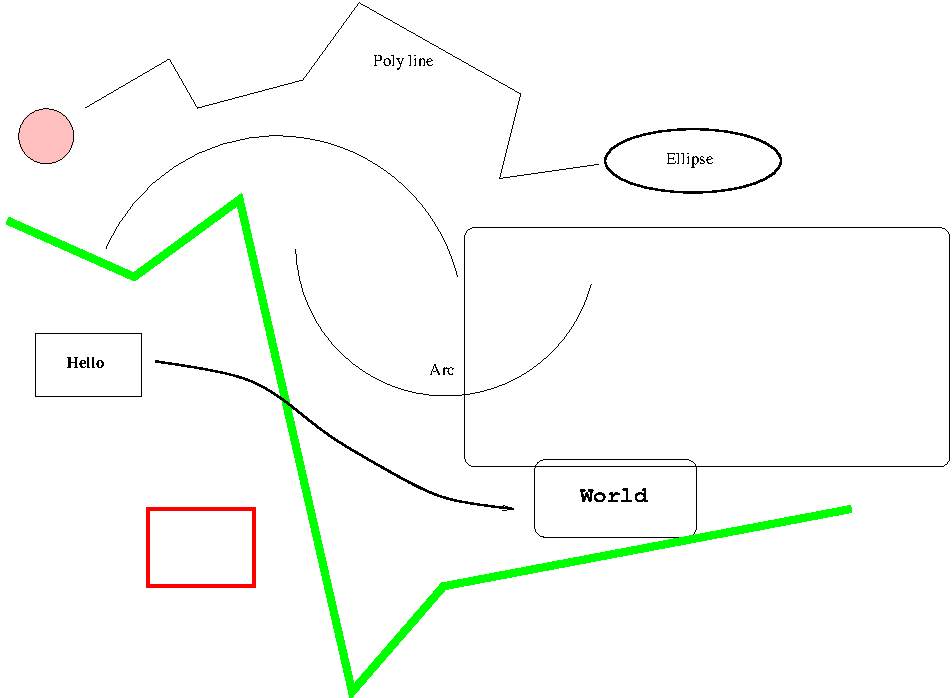
\includegraphics{figs/diagram.pdf}}
\caption{Example diagram drawn using \texttt{xfig}}
\label{xfig}
\end{figure}


\chapter{Evaluation}

\section{Printing and binding}

Use a ``duplex'' laser printer that can print on both sides to print
two copies of your dissertation. Then bind them, for example using the
comb binder in the Computer Laboratory Library.

\section{Further information}

See the Unix Tools notes at

\url{http://www.cl.cam.ac.uk/teaching/current-1/UnixTools/materials.html}


\chapter{Conclusion}

I hope that this rough guide to writing a dissertation is \LaTeX\ has
been helpful and saved you time.


%%%%%%%%%%%%%%%%%%%%%%%%%%%%%%%%%%%%%%%%%%%%%%%%%%%%%%%%%%%%%%%%%%%%%
% the bibliography
\addcontentsline{toc}{chapter}{Bibliography}
\bibliography{refs}

%%%%%%%%%%%%%%%%%%%%%%%%%%%%%%%%%%%%%%%%%%%%%%%%%%%%%%%%%%%%%%%%%%%%%
% the appendices
\appendix

\chapter{Latex source}

\section{diss.tex}
{\scriptsize\verbatiminput{diss.tex}}

\section{proposal.tex}
{\scriptsize\verbatiminput{proposal.tex}}

\chapter{Makefile}

\section{makefile}\label{makefile}
{\scriptsize\verbatiminput{makefile.txt}}

\section{refs.bib}
{\scriptsize\verbatiminput{refs.bib}}


\chapter{Project Proposal}

% Note: this file can be compiled on its own, but is also included by
% diss.tex (using the docmute.sty package to ignore the preamble)
\documentclass[12pt,a4paper,twoside]{article}
\usepackage[pdfborder={0 0 0}]{hyperref}
\usepackage[margin=25mm]{geometry}
\usepackage{graphicx}
\usepackage{parskip}
\begin{document}

\begin{center}
\Large
Computer Science Tripos -- Part II -- Project Proposal\\[4mm]
\LARGE
A Distributed Approach to Collaborative Live Music Performances\\[4mm]

\large
Elias Calocane, King's College

Originators: Elias Calocane, Sam Aaron and Martin Kleppmann

20 October 2017
\end{center}

\vspace{5mm}

\textbf{Project Supervisor:} Martin Kleppmann

\textbf{Project Adviser:} Sam Aaron

\textbf{Director of Studies:} Dr T.~G.~Griffin

\textbf{Project Overseers:} M.~P.~Fiore  \& T.~M.~Jones

% Main document

\section*{Introduction}

Making music using computers, is a well-established process. Digital Audio Workstation (DAW) software is available for users to create music on their machines using components such as real and virtual instruments, vocal tracks and other types of samples. In terms of collaborating, DAWs allow multiple users to synchronously work on a project, although it is convention for this to be done in the same location and machine.

In terms of composition or performance of music where users collaborate remotely (for example over a network), in both asynchronous and synchronous cases of contributions, the options are far more limited. One option for collaborative composition, is for collaborators to share project files and asynchronously build a musical piece e.g. via a network filesystem. However, this approach does not allow for several users to concurrently edit the files (in a synchronous fashion). Ableton use another (synchronous performance) approach through Ableton Link, an extension for their DAW and other Link-compatible software. Link allows musicians using compatible software to play in sync (live) whilst connected through a network -- by ensuring that all players adhere to a global sense of time through tempo synchronisation, beat alignment and phase synchronisation. However, Link requires that all collaborators are connected to the same local area network.

This project sets out to overcome the local network restrictions of Link and provide a Link-inspired functionality that works in a wide area network, whilst still focusing on the element of live performances by making use of Sonic Pi -- thus providing a synchronous and distributed method for musicians to collaborate.

A wide area approach naturally introduces challenges involving dealing with networking issues such as latency and jitter, routing messages through firewalls and NAT middleboxes, as well as (very critically) the problem of making sure everyone involved in the performance observes the same events in the same order. This distributed sense of coherence is vital to ensuring that everyone perceives the performance in the same way (so that it sounds the same for all users), and this coherence is the main focus of this project.

\section*{Starting Point}


Relevant Courses include Networking and Distributed/Concurrent Systems from Part IB.

Access to Ableton Link's developer resources (including GitHub repository with source code).

Access to the source code for Sonic Pi through GitHub.


\section*{Key Concepts}

\emph{These are the main concepts/technologies this project will try to bring together}

\Large
Link

\normalsize
\emph{Link is an open source networking library for music applications that allows users to play in sync by synchronising tempo, aligning beats and synchronising phase. Below is an explanation of the main concepts behind Link.}

\large
Tempo synchronisation

\normalsize
Tempo can be described as the rate at which a musical piece progresses, measured in beats per minute (BPM). To allow different musicians to play with each other in a coherent manner, it is essential that their contributions to the musical piece advance at the same rate, by making sure that all musicians adhere to the same predefined tempo.

\large
Beat alignment

\normalsize
Advancing at the same rate is not sufficient for contributions to a specific piece to sound coherent -- it is also essential that the beats occur at the same time (that they are aligned). In order to clarify what is meant by this, we adopt a numbering system for beats such that the first beat is denoted by number 1, the second by number 2, the third by number 3, etc. Beat alignment ensures that the difference between the beats of any two users, is always an integer, such that it is possible for one user to be at beat 4 whilst another is at beat 2, but it is not possible for third user to be at beat 2.5 (halfway between beat 2 and 3).

\large
Phase synchronisation

\normalsize
When dealing with loops or bars (consisting of a set number of beats) it is also useful to ensure that there is some consensus regarding the points at which they start and end. This is so that loops created by different users start/end at sensible places relative to each other. For loops of the same size, this means starting and finishing together (which may involve delaying the triggering of loops so they start in sync with others). For loops of different sizes, there may be more than one point at which a loop can be triggered -- for example a 4-beat loop can start either at the start or the middle of an 8-beat loop.

\Large
Open Sound Control (OSC)

\normalsize
Open Sound Control defines a message-based protocol that allows communication between different multimedia devices such as computers and synthesisers. On networks, OSC messages are most commonly transported as UDP packets. OSC messages can be used to encode descriptions of sounds (or musically related events) that can then be used in various scenarios. We will make use of OSC messages to communicate between Sonic Pi instances (being run on different machines by different users) to ensure that they all agree on which sounds to produce.

\Large
Sonic Pi

\normalsize
Sonic Pi defines a well-established language and software that allows users to produce music through live-coding. OSC messages are used within the software to describe music related events that need to be relayed to a speaker (through an audio synthesis platform called SuperCollider, integrated into Sonic Pi). Sonic Pi also defines temporal semantics which provide ways of reasoning about when sounds are produced by the software as well as making sure this occurs in a deterministic manner (or relaying to the user when that is not a possibility).


\section*{Structure}

\Large
Implementation

\normalsize
A user writes a script using Sonic Pi which generates OSC messages describing the sound they intend to make. These messages are then interpreted by the SuperCollider server to play the correct sound from the user's speakers. In the current implementation of Sonic Pi, these OSC messages flow only between the Sonic Pi process and SuperCollider running on the same machine. In this project we plan to extend Sonic Pi for distributed use by also transmitting these OSC messages over wide-area networks to other participants in the musical session. These messages need to be sent from each Sonic Pi instance to all other instances that are part of the performance so that other contributors are also able to hear the sounds that the original user intended to produce. A server will be used to setup a connection between Sonic Pi instances so that OSC messages can be transported between them.

Since we are focusing on a collaborative performance, it is vital that all users hear exactly the same sounds in the same order -- or in other words, that the lists of OSC messages interpreted by each user's SuperCollider server, are exactly the same. It is therefore important to account for aspects such as latency and jitter in the network to ensure that we are able to provide a consistent order of events for all users when they are all transmitting OSC messages to each other.

Sonic Pi schedules sounds to be played by SuperCollider ahead of time (the default schedule ahead time is 0.5 seconds). This is done to provide users a well-defined level of determinism describing the timing relationship between when an event described by a script is scheduled and its corresponding sound is played. This schedule ahead time gives us time to relay OSC messages over the network -- assuming latency is low enough and jitter issues are dealt with, we aim for these messages to reach all users before their respective sounds are expected to be played. When users all play together and their OSC messages have been exchanged, the data sent to each SuperCollider instance is the union of all the messages generated by the participants. We wish to sort these OSC messages by their scheduled timestamp (and schedule them) so that everyone observes the same message sequence.

\Large
Evaluation

\normalsize

We predict that it is possible to maintain a coherent musical collaboration through a wide area network if latency and jitter are below some threshold -- as mentioned above, Sonic Pi provides a scheduleAheadTime parameter set to 0.5s by default, and this parameter can be used to force Sonic Pi instances to adhere to the threshold we define. We will initially set our threshold to the default scheduleAheadTime, but will use network data from different sources (described below), as well as features from Link's Phase Synchronisation concept, to help define a suitable upper bound for the threshold.

We will test our hypothesis by emulating different network conditions using dummynet (or a similar tool). Using dummynet, we can control packet delay and jitter and investigate the effect they have on the coherence of a distributed music session, thus determining whether coherence is observed when conditions are under the threshold. We will measure coherence by comparing the sequences of OSC messages received by each SuperCollider instance -- looking at the events describing the sounds each user is about to play. If these sequences are identical, so that messages are in the correct order (before they are scheduled to be played), we will conclude that the session is in a coherent state. We will measure latency and packet loss rate in both the University network, and a home ISP to find out what kind of network conditions we are likely to encounter (on average) -- this will help guide the emulation of network conditions using dummynet, ensuring the system is able to deal with realistic scenarios. Using these findings, we will attempt to improve our implementation to automatically tune the scheduleAheadTime parameter of the separate Sonic Pi instances to adapt to different network conditions -- keeping scheduleAheadTime as low as possible so users experience the best possible response time (in audible terms) when submitting changes to their own scripts.

We aim to create different versions of the system using TCP and UDP and use the protocol that provides the best performance. We first need to determine how costly packet delay, jitter and packet loss are to the quality of the music session (in terms of coherence). We will measure how much adjusting these aspects individually (using dummynet) affects coherence -- for example, by examining the OSC messages received by all users in a session, and counting the number of messages that were observed in an incorrect order (or not at all). Protocol performance will then be rated using measurements of the latency, jitter and packet loss rate that the network experiences when using the protocols -- by comparing the performance measurements to their relative costs on session quality, we will be able to establish which protocol provides the better results.

\section*{Success Criteria}

Implement system allowing at least three users to setup a connection and play together using Sonic Pi i.e. allow users to write scripts describing sounds they wish to play as contributions to the performance, broadcast OSC messages describing these sounds to other members of a session, allow users to hear each other's contributions to the performance, propagate changes to contributions to all users in the session.

Ensure coherence of each user's notion of the performance -- so all users that are part of a performance hear the same thing. We wish to guarantee coherence for all users involved in a session when network conditions are acceptable i.e. when latency and jitter do not cause a delay that surpasses a defined threshold.

Ensure that when in a session, users' timelines don't drift relative to each other -- as the clocks rates of different users are likely to differ, we wish to prevent clock drift as this would eventually render users unable to react to each other's contributions (even when coherence holds). We wish to implement a clock synchronisation method and ensure it works by regularly comparing clock timestamps of users in a session.


\section*{Possible Extensions}

If I achieve my main goals early I shall try the following,

Integrate WebRTC into the project instead of using a server to provide a peer-to-peer implementation -- if such an approach were to reduce latency significantly, it may be possible to implement features such as making it possible for different users to update (different) aspects of the same sound at the same time (whilst still keeping a coherent view of events across all users).
Carrying out the evaluation steps for this new implementation would allow for a comparison between the original server-based and peer-to-peer approaches to the project.

Trying out different schemes for getting coherence.

\section*{Resources Required}


I will be primarily relying on the use of my own laptop for the project -- a laptop with an Intel Core i7 4720HQ Processor, 16GB RAM, 512GB SSD and NVIDIA GeForce GTX 960M GPU running Windows 10.

If my laptop should fail, I will use a MCS workstation in the Computer Laboratory.

I will run weekly backups to a personal USB stick as well as to GitHub and Google Drive.

\newpage
\section*{Timetable}


\begin{enumerate}

\item \textbf{Michaelmas weeks 2--4:} Read up on similar projects already out there and familiarise myself with Ableton Link's and Sonic Pi's source code and implementations.

\item \textbf{Michaelmas weeks 5--6:} Start first implementation of the server with first protocol (UDP or TCP). This initial implementation will be a simple echo server that will receive OSC messages from a Sonic Pi instance, and send them back.
\newline\textbf{Milestones:} Test echo server with connection to one Sonic Pi instance -- make sure it can send received messages back to Sonic Pi.

\item \textbf{Michaelmas weeks 7--8:} Finish the first implementation of the server. By this point I aim to be able to: setup a connection between (at least two) users, send and receive OSC messages from a Sonic Pi instance, schedule received OSC messages (so that a user will be able to hear the sound corresponding to the messages sent by another user).
\newline\textbf{Milestones:} Build server (with integrated clock synchronisation method).

\item \textbf{Michaelmas vacation:} Carry out alternative implementation of the server using second protocol. Start second implementation of the server for both protocols. Start planning dissertation chapters. Take measurements of latency and packet loss rate in home ISP.
\newline\textbf{Milestones:} Collect home ISP network data. Write draft of dissertation introduction.

\item \textbf{Lent weeks 0--2:} Finish the second implementation of the project. By this point I aim to be able to: provide some sense of consensus across all users -- this will involve merging the OSC messages produced by a user with those received from other users and doing so in a consistent manner for all instances that are part of the session.
\newline\textbf{Milestones:} Write progress report. Simulate session to test coherence and collect results for improvements. Write draft of preparation and implementation chapters.

\item \textbf{Lent weeks 3--5:} Run main experiments described in evaluation and achieve working project.
\newline\textbf{Milestones:} Test UDP vs TCP and collect results. Measure session coherence. Write draft of evaluation chapter.

\item \textbf{Lent weeks 6--8:} Absorb any incomplete work from the previous stages (if any of them were delayed). If possible, start integration of alternative WebRTC-based method of communication.
\newline\textbf{Milestones:} Write draft of conclusions chapter.

\item \textbf{Easter vacation:} Revise drafted chapters. Work on project extensions (optional).
\newline\textbf{Milestones:} Complete first version of dissertation.

\item \textbf{Easter term weeks 0--2:}  Carry out any further evaluation required, add content to chapters regarding any completed extension work.
\newline\textbf{Milestones:} Complete final version of dissertation.

\item \textbf{Easter term week 3:} Proof read - assuming no considerable delays were experienced in the previous stages.
\newline\textbf{Milestones:} Submit Dissertation.

\end{enumerate}

\end{document}


\end{document}
